\documentclass{jarticle}
\usepackage{robomech}
\usepackage[dvipdfmx]{graphicx}

\begin{document}
\makeatletter
\title{日本語表題:ゴシック体・14pt(欧文Arial・14pt)}
{―日本語副題:ゴシック体・12pt(欧文Arial・12pt)―}
{English Title: Times New Roman, 12pt}
{-Englsih Subtitle: Times New Roman, 10pt-}

\author{
\begin{tabular}{ll}
 \hspace{1zw}正\hspace{1zw}新宿大五朗 (機械大)& ○准\hspace{1zw} 渋谷次郎(ロボメカ電機)\\
 \hspace{1zw}学\hspace{1zw}東京 学(西大)& [日本語著者名:明朝体10pt]\\
 &\\
 \multicolumn{2}{l}{\small Daigoro SHINJUKU, Kikai University, daig\_shinj@kikai.ac.jp}\\
 \multicolumn{2}{l}{\small Jiro SHIBUYA, Robomec Electric Corporation}\\
 \multicolumn{2}{l}{\small Manabu TOKYO, Nishi University}\\
 \multicolumn{2}{l}{[\small Authors' names and Affiliations: Times New Roman, 9pt]}
\end{tabular}
}
\makeatother

\abstract{
\small
Papers submitted must be original, and previously unpublished. The responsibility for the contents of published articles rests solely with the authors and not the society. Copyright of the papers published belongs to the JSME (Japan Society of Mechanical Engineers). [Abstract: Times New Roman, 9pt, 100-150words]
}

\date{} % 日付を出力しない
\keywords{Robot, Manipulation,… (no more than five words) [Times New Roman, 9pt]}

\maketitle
\thispagestyle{empty}
\pagestyle{empty}

\small
\section{緒言(大見出し:ゴシック体・10pt・\protect\\ 強調文字・中央寄せ)}%===========================
本文:明朝体・9pt(欧文Times New Roman, 9pt),文字間隔は1行26文字程度,行間隔は4.2mm程度にして下さい.

\subsection{論文作成に関する注意事項を以下に示します.(中見出し:ゴシック体・9pt・強調文字・左寄せ)}%-----------
\begin{itemize}
	\item 用紙サイズ:A4(210×297mm)とします.
	\item 用紙マージン:上下25mm.日本語表題からKey Wordsまでの1段組の部分は,左右25mm以上空けて下さい.本文からは2段組とし,左右15mm,段間は6mmとします.
	\item 文字のフォント,大きさ:\reftab{tbl: table1}を参照下さい.
	\item 図の画質:300dpi以上の画質の高いものにして下さい.
	\item 図・表のタイトル:図のタイトルには「Fig.\# English title」,表のタイトルには「Table \# English title」という形式を用い,文中ではそれぞれ「図\#」,「表\#」という表現にして下さい.
	\item グラフの軸タイトル:各軸のタイトルに変数記号だけを記述するのは避けて下さい.\reffig{fig: fig1}に示すように,軸を表す語句ならびに単位を記入して下さい.
	\item 式:以下に示すように,右寄せで番号をふり,式は中央に配置して下さい.文中では「\refeqn{eqn: eq1}」と表現して下さい.
	
	\begin{equation}
		M\ddot{r}_{strl} + F_{frk} = Mg
		\label{eqn: eq1}
	\end{equation}

	\item 単位:SI単位系とします.
	\item 本文中に文献を引用する場合,引用を表す語句や文の後ろに文献番号(例えば\cite{Shinjuku98})を振って下さい.文献を主語や目的語などに用いる場合,「文献\cite{Shinjuku99}では,・・」などのようにして,番号のみの表現を避けて下さい.
	\item 連名の場合には講演発表者氏名の前に○印をつけて下さい.
	\item 作成した論文はPDFファイル形式に変換し,PDFファイルのみを学会本部へ提出して下さい.PDFファイルの提出は本講演会ホームページ記載のアップロードのページの指示に従って下さい.
\end{itemize}

※ ただし,PDFファイルの容量は2MB以下,論文のページ数は2頁以上4頁以下とします.なお,印刷原稿の提出は不要ですので,郵送しないで下さい.

※ 講演番号,講演会名,ページ番号は記載しないようにして下さい.


\begin{table}[tb]
 \caption{Type size and typefaces for papers}
 \label{tbl: table1}
 \centering
 \footnotesize
 \begin{tabular}{|p{7zw}|l|l|l|}
  \hline
	適用場所	&日本語	&欧文 \\\hline
	標準のフォント	&明朝体 9pt	&Times New Roman 9pt \\\hline
	日本語表題	&ゴシック体 14pt	&Arial 14pt \\\hline
	日本語副表題	&ゴシック体 12pt	&Arial 12pt \\\hline
	英語表題	&&Times New Roman 12pt \\\hline
	英語副表題	&&Times New Roman 10pt \\\hline
	日本語著者名	&明朝体 10pt &\\\hline
	英語著者名	&&Times New Roman 9pt \\\hline
	アブストラクト・キーワード	&&Times New Roman 9pt \\\hline
	大見出し	&ゴシック体 10pt	&Arial 10pt \\\hline
	中見出し	&ゴシック体 9pt	&Arial 9pt \\\hline
	図・表の番号・タイトル	 &&Times New Roman 9pt \\\hline
	文献	&明朝体 8pt	&Times New Roman 8pt \\
  \hline
 \end{tabular}
\end{table}

\begin{figure}[tb]
 \centering
  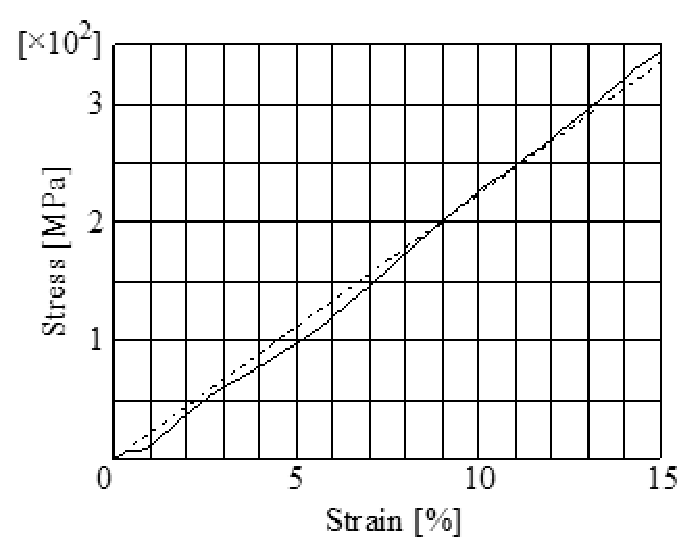
\includegraphics[height=38mm]{figs/fig1.eps}
  \vspace*{-4mm}
  \caption{Tensile stress-strain diagram}
  \label{fig: fig1}
\end{figure}


\footnotesize
\bibliographystyle{robomech}
\bibliography{main}

\normalsize
\end{document}
